\chapter{Disseny}
\label{cha:dessign}

En aquest cap\'{i}tol s'explica el disseny implementat per complir l'especificació del sistema. Es defineix la arquitectura del sistema, els patrons de dissenys emprats i les interfícies mes complexes. 

\section{Esquema general l\`{o}gic arquitect\'{o}nic del sistema}
A continuació expliquem el la arquitectura lògica dels components del sistema. La figura \ref{fig:archsoftware} \'{e}s un esquema s'aquesta arquitectura.\\

Els components de l'arquitectura son:

\begin{figure}[h!]
  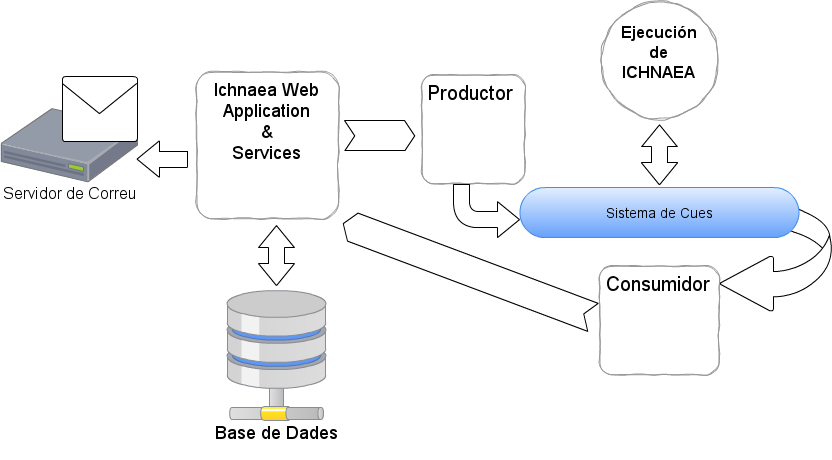
\includegraphics[scale=0.5]{img/design/ArchitectureSoftware.png}
  \caption{Arquitectura del sistema}
  \label{fig:archsoftware}
\end{figure}

\begin{itemize}
\item \textit{Ichnaea Web Application \& Services}: \'{e}s el \textit{core} de la aplicaci\'{o} i dels serveis HTTP. Es el codi i la aplicació desenvolupada. Es el principal responsable del projecte.
\item Servidor de correu \'{e}s el servidor SMTP per enviar correus electr\`{o}nics als usuaris.
\item Productor-Cua-Consumidor \'{e}s el sistema de cues. Expliquem el paradigma al cap\'{i}tol \ref{sec:queue_system_overview}. La funci\'{o} \'{e}s gestionar els inicis, fluxos i finals d'execucions de Ichnaea.
\item La base de dades \'{e}s on es guarden els continguts, els models de dades i els resultats.
\item El sistema de fitxers \'{e}s on es guarden els resultats en format binari dels entrenaments per usar amb les prediccions.
\end{itemize}

\section{Patr\'{o} de disseny}
Per la implementaci\`{o} del sistema web s'han usat un disseny per capes: presentaci\'{o}, domini i persistència de dades. S'han seleccionat els seguents patrons conforme a complir els requeriments especificats.
  \begin{itemize}
  \item Model-Vista-Controlador amb controlador frontal
  \item Capa de Servei
  \item Injecci\'{o} de depend\`{e}ncies
  \item Repositori de model de dades
  \item Capa de mapejat de dades
  \item View template
  \item Interfícies enriquides amb servei webs
  \end{itemize}
A continuació expliquem detalladem cadascun d'aquests patrons.

\subsection{Esquema del disseny}
Per tal de donar una visió general del patrons de disseny usats, dediquem aquesta secció a un diagrama esquematic dels patrons usats.\\

La figura \ref{fig:dessignpatters} dona una visió general de la integració i les responsabilitats de cadascun dels patrons.
\begin{figure}[H]
  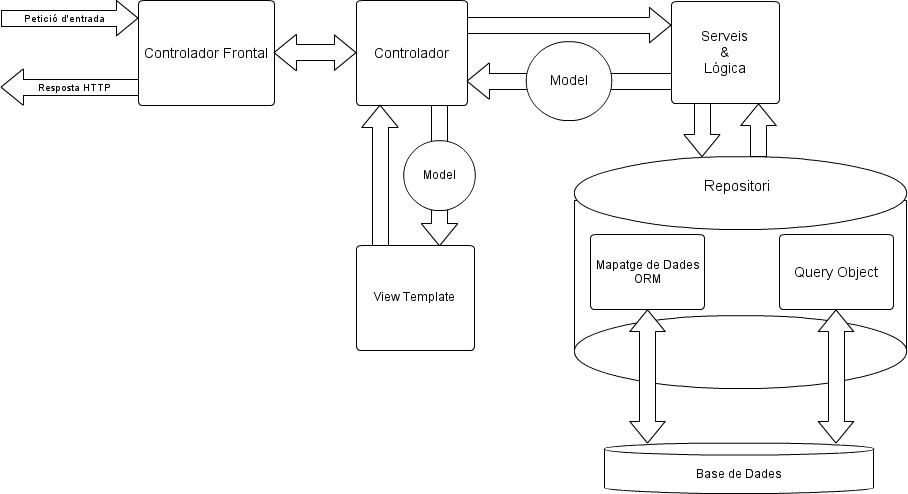
\includegraphics[scale=0.5]{img/design/IchnaeaPatterns.png}
  \caption{Patrons de disseny}
  \label{fig:dessignpatters}
\end{figure}

A continuació expliquem detalladament els patrons de disseny i la integracio entre ells.

\subsection{Explicaci\'{o} del disseny}
\subsubsection{Model-Vista-Controlador amb controlador frontal}
El patró Model-Vista-Controlador \'{e}s un disseny t\'{i}pic en les aplicacions web on:
\begin{itemize}
\item el \textbf{model} \'{e}s una representaci\'{o} de les dades.
\item la \textbf{vista} transforma el model a un format visible i llegible.
\item el \textbf{controlador} rep les peticions i dona les sortides.
\end{itemize}
El controlador frontal \'{e}s una variació del controlador que centralitza totes les peticions i les re-dirigeix cap als controladors corresponents. La principal avantatge d'aquesta \'{e}s la centralització de les peticions per en un únic punt, augmentem la re-usabilitat del codi i millorem la gestió de la seguretat.

\subsubsection{Injecció de dependencies}
L'arquitectura \textbf{MVC} separa la capa de presentaci\'{o} de la l\`{o}gica de domini. La capa de presentaci\'{o} accedeix a la capa de domini mitjançant serveis, injectant depend\'{e}ncies. \\

La \textbf{injecci\'{o} de depend\'{e}ncies} \'{e}s un patr\'{o} a on es subministren objectes a una classe en lloc de ser la classe qui crea els objectes.\cite{dependency_injection} Les avantatges de usar DI(''dependency injection'') son:
\begin{itemize}
\item Codi m\'{e}s f\`{a}cil de mantenir, extendre o modificar
\item Desenvolupament guiat per proves (Test Driven Development o TDD en angl\'{e}s)
\item DI ens obliga a planejar una mica millor les nostres depend\`{e}ncies; decidim si una classe realment necessita d'un altre objecte per realitzar la seva funció.
\end{itemize}

\subsubsection{Repositori de model de dades}
En la \textbf{capa de serveis} cont\'{e} la l\'{o}gica de Ichnaea. Accedeixen a les dades mitjançant \textbf{repositoris} d'objectes. Els \textbf{repositoris} son mediadors entre el domini i les dades persistents. Els repositoris retornen entitats i/o collecions d'entitats de la l\'{ogica} de domini. \\

El \textbf{mapatge de dades} ORM(''Object Relational Mapping''), mapatge objecte-relacional, \'{e}s un patr\'{o} de disseny(encara que alguns enginyers els agrada dir que \'{e}s una tècnica de programaci\'{o} i a uns altres una tecnologia) que estableix una relaci\'{o} directe entre les entitats i la dades persistents.\cite{orm}

\section{Disseny d'interf\'{i}cies}
\label{sec:dessigninterfaces}
En el disseny de les interfícies, es pretén definir com serà la part del sistema que interactua amb l’usuari. Consisteix en definir els mecanismes amb els quals els usuaris podran interactuar amb el sistema i la manera de mostrar la informació a l’usuari.\\
\subsection{Disseny principal}
A continuació es detalla la estructura estètica de la aplicació.
DIAGRAMA
ESQUEMA DEL MENU
El menú serà condicional als permisos de l'usuari que estigui usant. La jerarquia del menu es la seguent:
\begin{itemize}
\item Logo
\item Matrius
 \begin{itemize}
 \item Les meves matrius
 \item Crear una matriu
  \end{itemize}
\item Entrenaments
 \begin{itemize}
 \item Els meus entrenaments
 \item Crear un entrenament
 \end{itemize} 
\item Prediccions
 \begin{itemize}
 \item Les meves prediccions
 \item Crear una predicció
 \end{itemize} 
\item Dades de Ichnaea 
 \begin{itemize}
 \item Variables del sistema
 \item Fitxers
 \item Matrius
 \item Llista de entrenaments predictibles
 \end{itemize} 
\item Administració: Solament disponible per usuaris administradors
\begin{itemize}
\item Usuaris
\item Crear una variable
\item Eines administratives de control de cues
\item Llista d'entrenaments
\item Llista de prediccions
\end{itemize}
\item Usuari
 \begin{itemize}
 \item Casa de l'usuari
 \item Canvi de contrasenya
 \item Desconectar-se
 \end{itemize}
\end{itemize}

\subsection{Interf\'{i}cie de configuraci\'{o} de matrius}
El disseny d'interfícies per les configuracions de les matrius es basa en funcionalitats enriquides\cite{ria}. Per dotar de funcionalitats a les interfícies webs s'utilitza peticions asíncrones.\\ 

Per complir aquest requeriment s'ha de dissenyar una llibreria per atendre les peticions asíncrones i desenvolupar funcionalitats per atendre les respostes a aquestes peticions. A continuaci\'{o} es descriuen les interf\'{i}cies m\'{e}s complexes: les responsables de la configuraci\'{o} de les matrius.

\subsubsection{Interf\'{i}cie de configuraci\'{o} de matrius}
Les funcionalitats enriquides que han de complir son:
\begin{itemize}
\item Carrega de conjunt de fitxers segons les variables.
\item Guardar la configuració de una columna: alias, variable i conjunt de fitxers.
\item Desplegar un calendari per seleccionar una data i assignar-la a una mostra.
\item Desplegar un selector obert de possibles valors de tots els orígens que estiguin especificats a les mostres.
\item Actualitzar el valor d'una mostra i d'una variable.
\item Permetre la mobilitat per la matriu fixant les capçaleres de les columnes i les files.
\item Adaptar-se a les dimensions de la pantalla.
\end{itemize}

A la figura \ref{fig:interfacematrixconf} s'especifica el disseny de la interfície de configuraci\'{o} de matrius.

\begin{figure}[H]
  \centering
  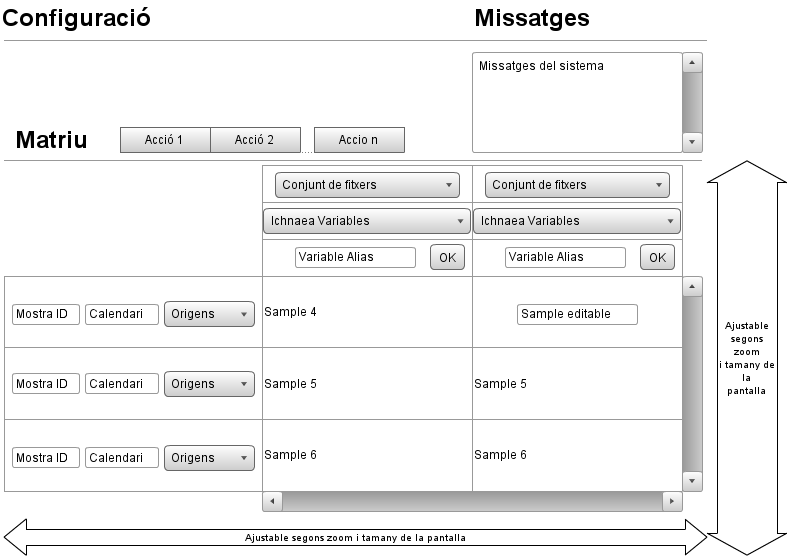
\includegraphics[scale=0.5]{img/design/Interficiedeconfiguracio.png}
  \caption{Interfície de configuració de matrius}
  \label{fig:interfacematrixconf}
\end{figure}


\subsubsection{Interf\'{i}cie de configuraci\'{o} de matrius de predicció}
Les funcionalitats enriquides que han de complir:
\begin{itemize}
\item Guardar la configuració de una columna: alias i assignació d'una columna entrenada.
\item Desplegar un calendari per seleccionar una data i assignar-la a una mostra.
\item Desplegar un selector obert de possibles valors de tots els orígens que estiguin especificats a les mostres.
\item Actualitzar el valor d'una mostra i d'una variable.
\item Adaptar-se a les dimensions de la pantalla.
\end{itemize}

A la figura \ref{fig:interfacematrixpredictionconf} s'especifica el disseny de la interfície de configuraci\'{o} de matrius de prediccions.

\begin{figure}[H]
  \centering
  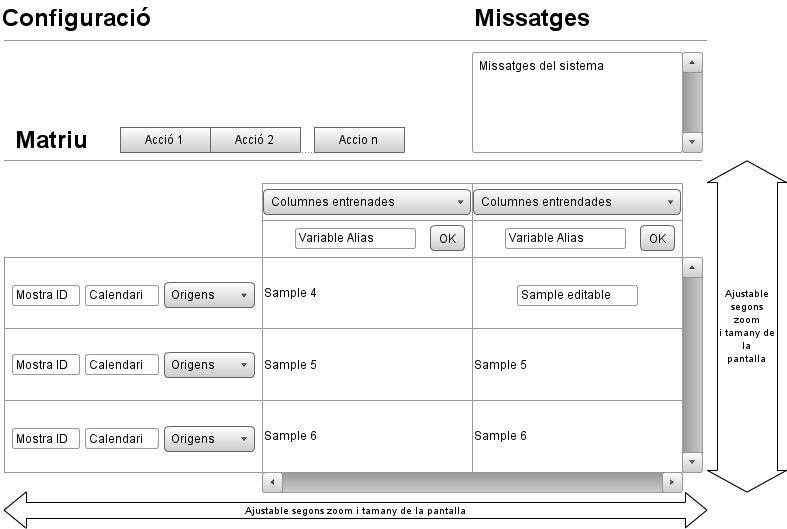
\includegraphics[scale=0.5]{img/design/Interficiedeconfiguraciopredi.png}
  \caption{Interfície de configuració de matrius de prediccions}
  \label{fig:interfacematrixpredictionconf}
\end{figure}
